\title{A Very Simple Document}
\author{
        Vitaly Surazhsky, Yossi Gil
}
\date{\today}

\documentclass[12pt]{article}

\begin{document}
\maketitle

\begin{abstract}
This is the paper's abstract \ldots
\end{abstract}

\section{Introduction}
This is time for all good men to come to the aid of their party!

\paragraph{Outline}
The remainder of this article is organized as follows.
Section~\ref{previous work} gives account of previous work.
Our new and exciting results are described in Section~\ref{results}.
Finally, Section~\ref{conclusions} gives the conclusions.

\section{Materials and Methods}
\label{previous work}
A much longer \LaTeXe{} example was written by Gil~\cite{Gil:02}.

\section{Results}
\label{results}
In this section we describe the results.

\begin{figure}
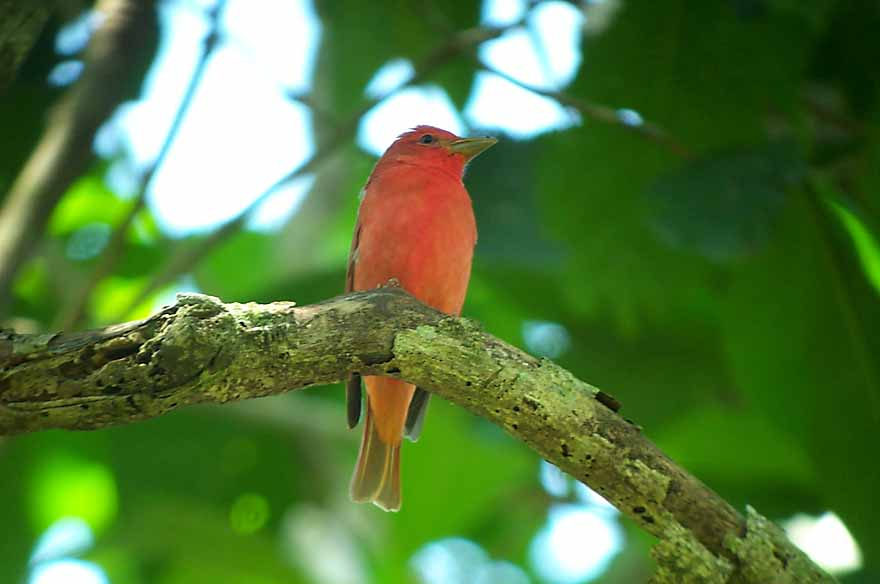
\includegraphics{summer_tanager_3_B.jpg}
\caption{this is a summer tanager.}
Here we provide a lot of witty repartee about the figure.
\end{figure}

\section{Discussion}
\label{conclusions}
We worked hard, and achieved very little.

\section{Acknowledgments}
We wish to thank you for taking your precious time to read this drivel.

\bibliographystyle{abbrv}
\bibliography{simple}

\end{document}
This is never printed
